\documentclass[aspectratio=169,10pt]{beamer}
% =============================================================================
% Every number on these slides is a macro from presentation/numbers.tex, which
% presentation/make_figures.py regenerates from
%     tables/*.csv                    (frozen authoritative tables)
%     code_hardened/results/*.json    (verification runs)
% Nothing on a slide is hand-typed; rerun make_figures.py and rebuild.
% Every figure is generated by the same script into presentation/figures/.
% =============================================================================

\usepackage{iftex}
\ifPDFTeX
  \usepackage[T1]{fontenc}
  \usepackage[utf8]{inputenc}
\fi

\usepackage{lmodern}
\usetheme{Madrid}

\usepackage{amsmath,amssymb}
\usepackage{booktabs}
\usepackage{array}
\usepackage{graphicx}
\usepackage{tikz}

\definecolor{brandblue}{RGB}{51,51,178}
\colorlet{mainblue}{brandblue}
\colorlet{darkblue}{brandblue!62!black}

\definecolor{cMain}{HTML}{1F2937}
\definecolor{cBlue}{HTML}{185FA5}
\definecolor{cRed}{HTML}{A32D2D}
\definecolor{cGreen}{HTML}{27500A}
\definecolor{cOrange}{HTML}{854F0B}
\definecolor{cGrey}{HTML}{5F5E5A}

\setbeamercolor{normal text}{fg=cMain}
\setbeamercolor{structure}{fg=mainblue}
\setbeamercolor{frametitle}{bg=mainblue,fg=white}
\setbeamercolor{palette primary}{bg=mainblue,fg=white}
\setbeamercolor{palette secondary}{bg=darkblue,fg=white}
\setbeamercolor{palette tertiary}{bg=darkblue,fg=white}
\setbeamercolor{palette quaternary}{bg=darkblue,fg=white}
\setbeamercolor{title}{fg=white,bg=mainblue}
\setbeamercolor{subtitle}{fg=white}
\setbeamercolor{alerted text}{fg=cRed}

\setbeamertemplate{navigation symbols}{}
\setbeamertemplate{blocks}[rounded][shadow=false]
\setbeamertemplate{itemize item}{\raisebox{0.15ex}{\scriptsize$\bullet$}}
\setbeamertemplate{itemize subitem}{\raisebox{0.15ex}{\tiny$\circ$}}

\setbeamerfont{title}{size=\LARGE}
\setbeamerfont{subtitle}{size=\large}
\setbeamerfont{block body}{size=\footnotesize}
\setbeamerfont{block title}{size=\small}
\setbeamerfont{itemize/enumerate body}{size=\footnotesize}
\setbeamerfont{itemize/enumerate subbody}{size=\scriptsize}
\setlength{\leftmargini}{1.15em}

\graphicspath{{./figures/}{../figures/}{../report/figures/}{./}}

\newcommand{\epsr}{\varepsilon_r}
\newcommand{\epseff}{\varepsilon_{\mathrm{eff}}}
\newcommand{\Cair}{C_{\mathrm{air}}}
\newcommand{\Zzero}{Z_0}
\newcolumntype{L}[1]{>{\raggedright\arraybackslash}p{#1}}
% Generated by presentation/make_figures.py -- do not edit by hand.
% Every number on the slides comes from tables/*.csv or code_hardened/results/*.json.

\newcommand{\CRef}{120.467}
\newcommand{\CRefPOne}{120.4673}
\newcommand{\CRefPTwo}{120.4670}
\newcommand{\RefAgree}{2.9\times10^{-6}}
\newcommand{\CFinal}{120.620}
\newcommand{\CFinalAbs}{0.153}
\newcommand{\ErrSeven}{0.127}
\newcommand{\ErrSix}{0.282}
\newcommand{\DeltaSeven}{0.156}
\newcommand{\DofSeven}{362{,}112}
\newcommand{\DofFive}{22{,}944}
\newcommand{\CAir}{35.968}
\newcommand{\CAirRef}{35.946}
\newcommand{\OrderPOne}{1.16}
\newcommand{\OrderPTwo}{1.15}
\newcommand{\GradedDof}{139{,}426}
\newcommand{\GradedErr}{0.017}
\newcommand{\GradedRatio}{7.6}
\newcommand{\GradedDofFrac}{39}
\newcommand{\TolDisc}{6.3\times10^{-3}}
\newcommand{\EpsEff}{3.3535}
\newcommand{\EpsRef}{3.3513}
\newcommand{\EpsErr}{0.07}
\newcommand{\ZFinal}{50.642}
\newcommand{\ZRef}{50.690}
\newcommand{\ZErrAbs}{0.048}
\newcommand{\ZErrPct}{0.09}
\newcommand{\ZHJ}{50.201}
\newcommand{\ZIPC}{49.393}
\newcommand{\ZBenchGap}{0.81}
\newcommand{\CheckCount}{23}
\newcommand{\TruncThree}{2.49}
\newcommand{\TruncFive}{0.71}
\newcommand{\TruncEight}{0.18}
\newcommand{\TruncFine}{0.036}
\newcommand{\RatioChange}{1.23}


\title[Microstrip FEM]{2D Finite Element Analysis of a Microstrip Line}
\subtitle{Capacitance and impedance, with a measured error}
\author[Project 2]{\texorpdfstring{Group C\\[0.4em]
  {\small Chuqiao Tang (2360692), Jinyu Ma (2363433)}\\
  {\small Muqing Xu (2362900), Shuoran Fu (2362626)}\\
  {\small Taiqi Zhang (2363684), Yujia Ding (2362094)}}{Group C: Chuqiao Tang, Jinyu Ma, Muqing Xu, Shuoran Fu, Taiqi Zhang, Yujia Ding}}
\institute[MTH321 Project 2]{MTH321 Numerical PDEs --- Project 2}
\date[October 2026]{October 2026}


% Unboxed text groups: bold headings replace repeated blue panels.
\newenvironment{plainsection}[1]{%
  \par\vspace{0.6ex}\begingroup\footnotesize
  {\small\bfseries #1\par}\vspace{0.45ex}%
}{\par\endgroup\vspace{0.8ex}}
\setbeamerfont{block title alerted}{size=\small,series=\bfseries}

\begin{document}

\maketitle

% ---------------------------------------------------------------------
\section{What we have to deliver}
% ---------------------------------------------------------------------

\begin{frame}{A number, and how wrong it is}
  \begin{columns}[T]
    \begin{column}{0.50\textwidth}
      \begin{plainsection}{What is required}
        \begin{itemize}
          \item \textbf{Capacitance per unit length} of the cross-section.
          \item The \textbf{all-air capacitance} on the \textbf{same mesh}.
          \item $\epseff$ and $\Zzero$ from that matched pair.
        \end{itemize}
      \end{plainsection}
    \end{column}
    \begin{column}{0.46\textwidth}
      \begin{plainsection}{What would not be enough}
        \begin{itemize}
          \item One FEM number that looks close to $50\,\Omega$.
          \item Agreement with an empirical formula only.
          \item Calling the result converged because two meshes agree.
        \end{itemize}
      \end{plainsection}
    \end{column}
  \end{columns}
  \vspace{0.7em}
  \begin{alertblock}{Takeaway}
    The deliverable is a number together with the distance from its limit.
  \end{alertblock}
\end{frame}

% ---------------------------------------------------------------------
\section{Model and discretisation}
% ---------------------------------------------------------------------

\begin{frame}{The cross-section and the equation}
  \begin{columns}[T]
    \begin{column}{0.56\textwidth}
      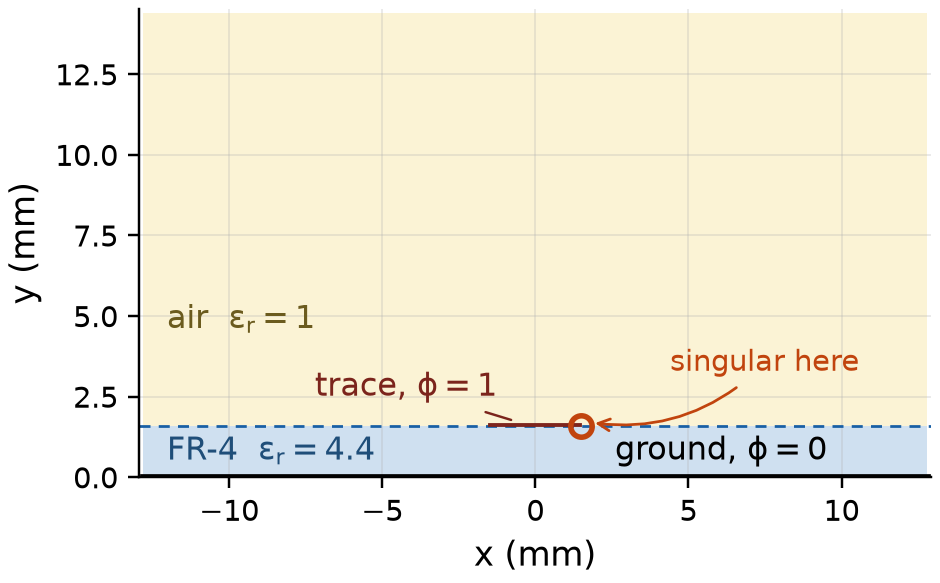
\includegraphics[width=\linewidth]{fig01_geometry.png}
    \end{column}
    \begin{column}{0.40\textwidth}
      \begin{plainsection}{Electrostatic model}
        \[
          -\nabla\cdot(\varepsilon\nabla\phi)=0
        \]
        \[
          \phi=1\,\mathrm{V}\ \text{on the trace},\qquad
          \phi=0\ \text{on the ground}
        \]
        Zero normal flux on the artificial top and side walls.
      \end{plainsection}
      \begin{plainsection}{Dimensions}
        $H=1.6\,\mathrm{mm}$, $w=3.0\,\mathrm{mm}$,
        $t=0.035\,\mathrm{mm}$, substrate $\epsr=4.4$.
      \end{plainsection}
    \end{column}
  \end{columns}
  \begin{alertblock}{Takeaway}
    The field is singular where the conductor edge ends on the dielectric interface.
  \end{alertblock}
\end{frame}

\begin{frame}{Weak form and $P_1$ elements}
  \begin{plainsection}{Weak problem}
    Find $\phi\in V_g$ with
    $\displaystyle\int_{\Omega}\varepsilon\nabla\phi\cdot\nabla v\,d\Omega=0$
    for every $v\in\mathcal V$.
  \end{plainsection}
  \begin{columns}[T]
    \begin{column}{0.48\textwidth}
      \begin{plainsection}{Discretisation}
        \begin{itemize}
          \item Conforming triangles, \textbf{linear shape functions}.
          \item The trace volume is excluded; \textbf{Dirichlet nodes are eliminated}.
          \item \textbf{Positive} $\varepsilon$ makes the free system SPD.
          \item Capacitance from the energy, $C=2U/V_0^2$.
        \end{itemize}
      \end{plainsection}
    \end{column}
    \begin{column}{0.48\textwidth}
      \begin{plainsection}{Interface}
        Potential is continuous and the normal flux balance holds in the
        \textbf{weak} sense only. Discrete fluxes need not match pointwise
        across an edge.
      \end{plainsection}
    \end{column}
  \end{columns}
  \begin{alertblock}{Takeaway}
    A small residual proves the linear system was solved, not that the mesh is adequate.
  \end{alertblock}
\end{frame}

% ---------------------------------------------------------------------
\section{Is the solver right?}
% ---------------------------------------------------------------------

\begin{frame}{\CheckCount{} analytic checks, one verdict}
  \begin{columns}[T]
    \begin{column}{0.56\textwidth}
      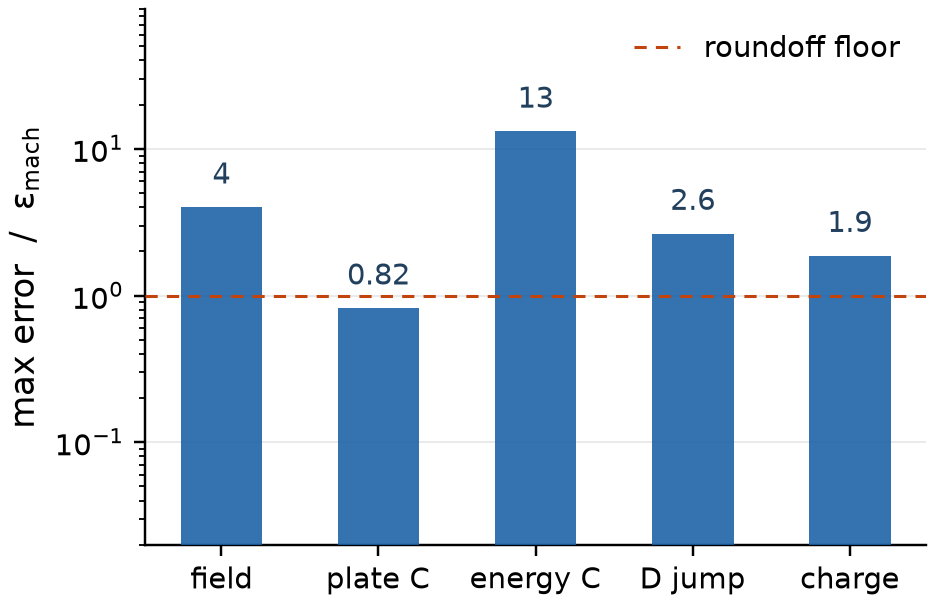
\includegraphics[width=\linewidth]{fig02_checks.png}
    \end{column}
    \begin{column}{0.40\textwidth}
      \begin{plainsection}{What is checked}
        \begin{itemize}
          \item Uniform field against $\phi=y/d$, for $\epsr=1$ and $4.4$.
          \item $C$ against $\varepsilon_0\epsr A/d$ and a two-layer series.
          \item Normal $D$ continuous across the interface.
          \item Charge balance and zero flux on the far walls.
          \item Symmetry, definiteness, monotone energy under refinement.
        \end{itemize}
      \end{plainsection}
      \begin{plainsection}{Result}
        All pass; the worst error is $\approx 13\,\varepsilon_{\rm mach}$.
      \end{plainsection}
    \end{column}
  \end{columns}
  \begin{alertblock}{Takeaway}
    Assembly and extraction are exact to roundoff, so every error left is discretisation.
  \end{alertblock}
\end{frame}

% ---------------------------------------------------------------------
\section{How accurate is M7?}
% ---------------------------------------------------------------------

\begin{frame}{Two elements, two codes, one limit}
  \begin{columns}[T]
    \begin{column}{0.54\textwidth}
      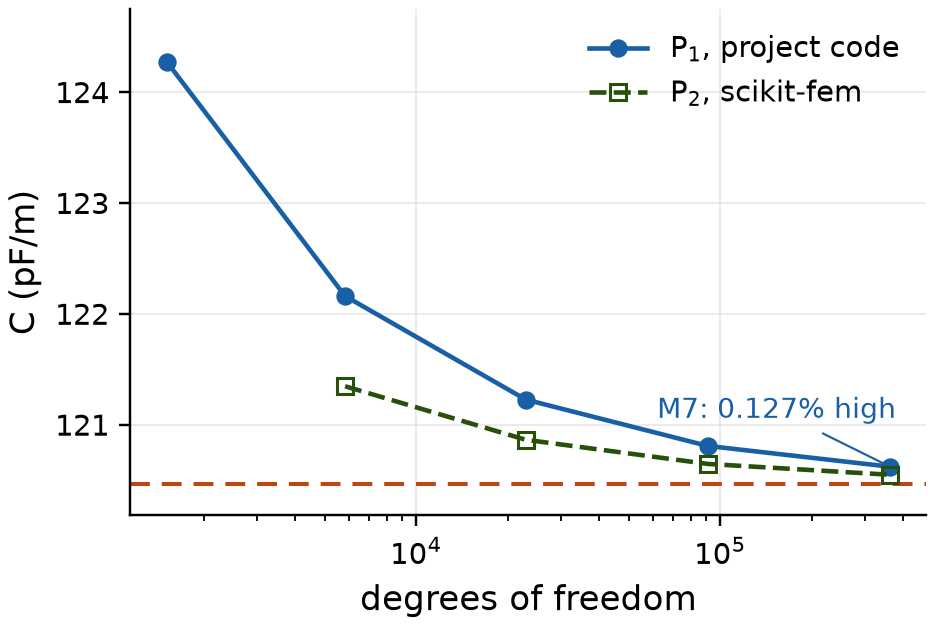
\includegraphics[width=\linewidth]{fig03_reference.png}
    \end{column}
    \begin{column}{0.42\textwidth}
      \begin{plainsection}{Two independent routes}
        \begin{itemize}
          \item The project's $P_1$ sequence, \textbf{Richardson extrapolated}.
          \item An independent scikit-fem $P_2$ solve on the \textbf{same mesh}es.
        \end{itemize}
        \[
          \CRefPOne \ \text{vs}\ \CRefPTwo\ \mathrm{pF/m}
        \]
        They agree to $\RefAgree$ relative.
      \end{plainsection}
      \begin{plainsection}{Reference adopted}
        $C_{\rm ref}=\CRef\,\mathrm{pF/m}$.
      \end{plainsection}
    \end{column}
  \end{columns}
  \begin{alertblock}{Takeaway}
    With a reference, an error can be measured instead of guessed.
  \end{alertblock}
\end{frame}

\begin{frame}{The old metric measured the wrong thing}
  \begin{columns}[T]
    \begin{column}{0.56\textwidth}
      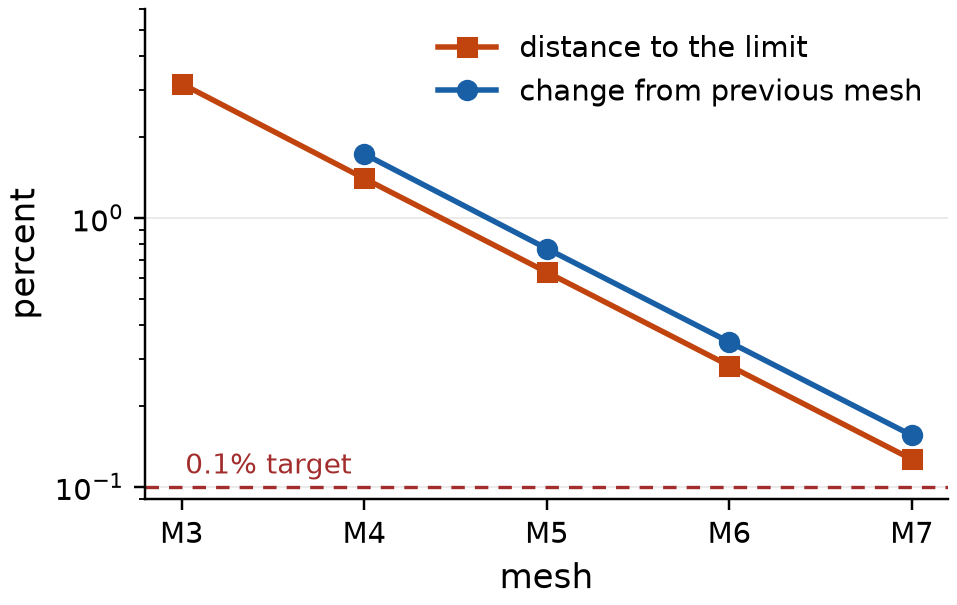
\includegraphics[width=\linewidth]{fig04_metric.png}
    \end{column}
    \begin{column}{0.40\textwidth}
      \begin{plainsection}{Two different questions}
        \begin{itemize}
          \item Change from M6 to M7: $\DeltaSeven\%$.
          \item Distance from the limit at M7: $\ErrSeven\%$.
        \end{itemize}
      \end{plainsection}
      \begin{plainsection}{Why they differ}
        For order $p$ the change is $(2^{p}-1)$ times the error, here
        $2^{1.16}-1=\RatioChange$. A shrinking change bounds nothing
        without knowing $p$.
      \end{plainsection}
    \end{column}
  \end{columns}
  \begin{alertblock}{Takeaway}
    M7 is $\ErrSeven\%$ from the limit, so the $0.1\%$ target is missed --- it is not converged.
  \end{alertblock}
\end{frame}

\begin{frame}{Quadratic elements do not buy an order}
  \begin{columns}[T]
    \begin{column}{0.54\textwidth}
      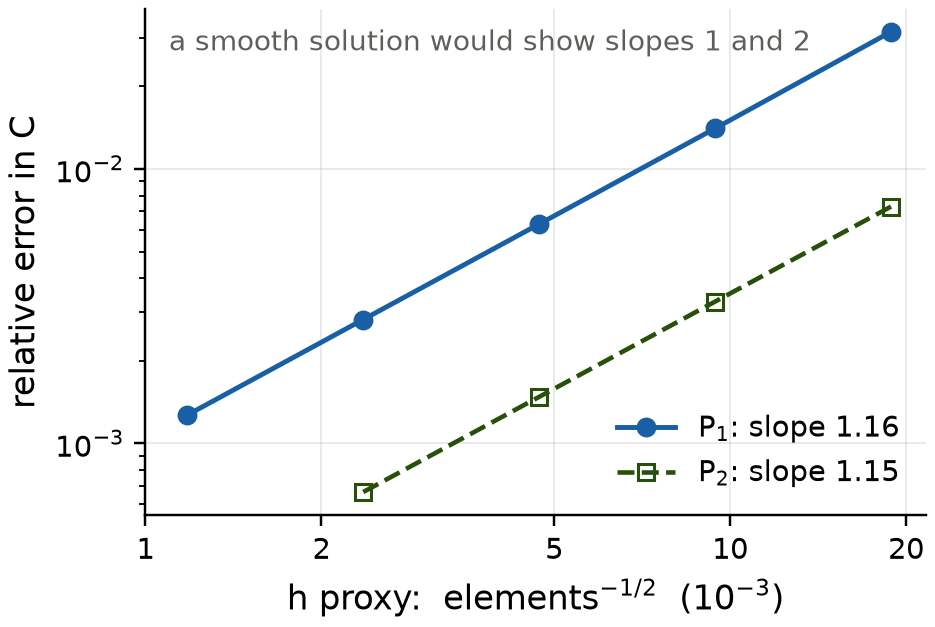
\includegraphics[width=\linewidth]{fig05_order.png}
    \end{column}
    \begin{column}{0.42\textwidth}
      \begin{plainsection}{Fitted slopes}
        \begin{tabular}{@{}lrr@{}}
          \toprule
          Family & DOF range & slope\\
          \midrule
          $P_1$ & 1.5k--362k & $\OrderPOne$\\
          $P_2$ & 5.8k--362k & $\OrderPTwo$\\
          \bottomrule
        \end{tabular}
      \end{plainsection}
      \begin{plainsection}{Diagnosis}
        Doubling the polynomial degree leaves the rate unchanged, so the
        limit is not the basis. The fitted field exponent near the corner is
        $0.54$, giving an energy error of order $2\times0.54\approx1.1$.
      \end{plainsection}
    \end{column}
  \end{columns}
  \begin{alertblock}{Takeaway}
    The order is set by the corner, so uniform refinement is the wrong tool.
  \end{alertblock}
\end{frame}

% ---------------------------------------------------------------------
\section{What fixes it}
% ---------------------------------------------------------------------

\begin{frame}{Corner grading restores the order}
  \begin{columns}[T]
    \begin{column}{0.56\textwidth}
      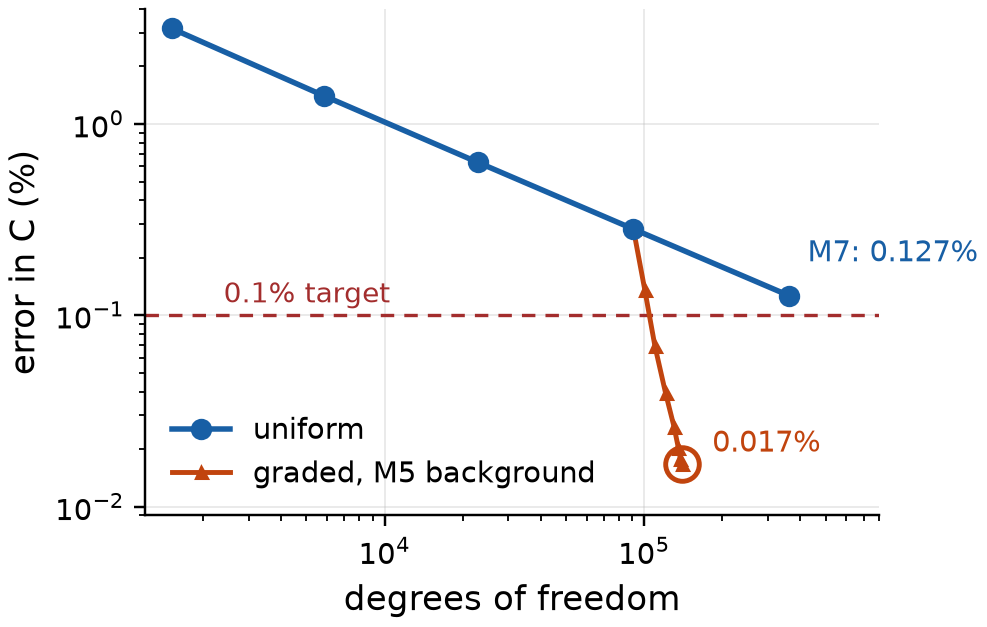
\includegraphics[width=\linewidth]{fig06_graded.png}
    \end{column}
    \begin{column}{0.40\textwidth}
      \begin{plainsection}{Same model, graded partition}
        Geometric refinement around the two trace ends on fixed background
        meshes M2 to M5.
      \end{plainsection}
      \begin{plainsection}{Result on the M5 background}
        \begin{tabular}{@{}lr@{}}
          \toprule
          & value\\
          \midrule
          DOF & $\GradedDof$\\
          error & $\GradedErr\%$\\
          vs M7 & $\GradedRatio\times$ better\\
          cost & $\GradedDofFrac\%$ of M7\\
          \bottomrule
        \end{tabular}
      \end{plainsection}
    \end{column}
  \end{columns}
  \begin{alertblock}{Takeaway}
    The plateau falls fourfold per background level, so the remaining error is $h^2$ again.
  \end{alertblock}
\end{frame}

\begin{frame}{Where the extra elements go}
  \begin{columns}[T]
    \begin{column}{0.55\textwidth}
      \centering
      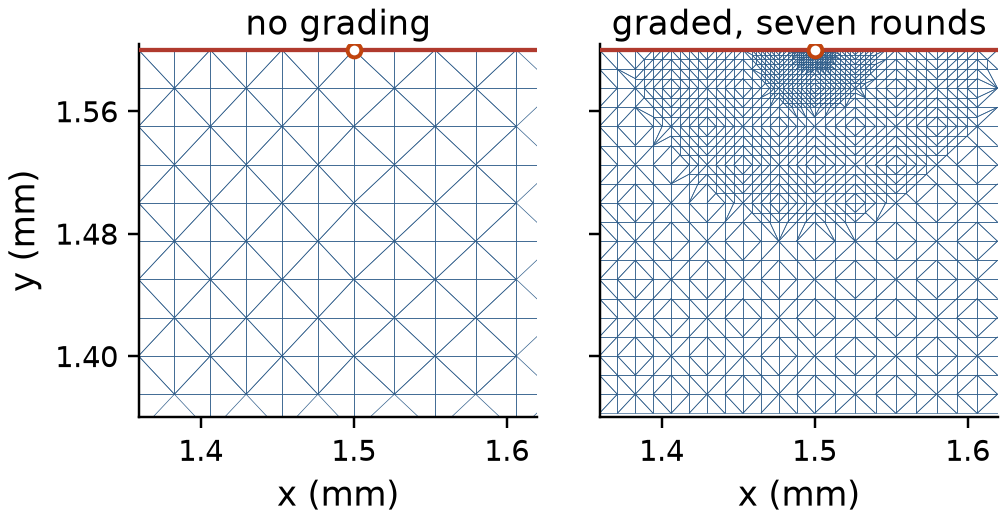
\includegraphics[width=\linewidth]{fig07_mesh.png}\\[-0.2em]
      {\scriptsize The same M5 background, seen near the right trace end.}
    \end{column}
    \begin{column}{0.42\textwidth}
      \begin{plainsection}{What changed}
        \begin{itemize}
          \item Elements are marked by \textbf{distance to the corner} and refined.
          \item The far field and the middle of the trace keep their coarse mesh.
          \item The operator, the boundary conditions and $C=2U/V_0^2$ are identical.
        \end{itemize}
      \end{plainsection}
      \begin{plainsection}{Cost}
        The solve stays a sparse direct solve; only the unknowns near the
        corner grow.
      \end{plainsection}
    \end{column}
  \end{columns}
  \begin{alertblock}{Takeaway}
    Grading changes the partition, not the equations --- so it is a choice we may make.
  \end{alertblock}
\end{frame}

\begin{frame}{The linear solver is not the bottleneck}
  \begin{columns}[T]
    \begin{column}{0.54\textwidth}
      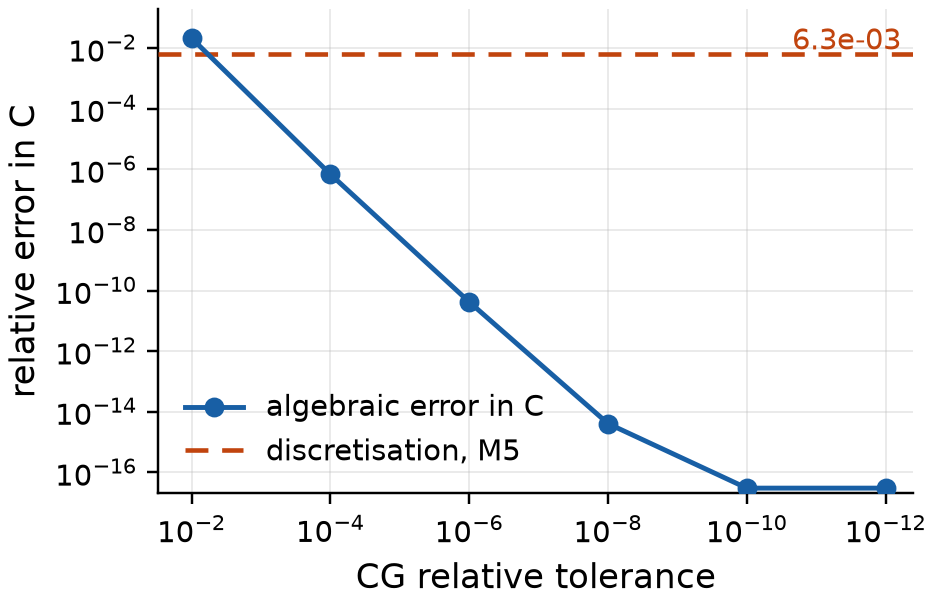
\includegraphics[width=\linewidth]{fig08_tolerance.png}
    \end{column}
    \begin{column}{0.42\textwidth}
      \begin{plainsection}{Tolerance ladder on M5}
        \begin{itemize}
          \item Conjugate gradients from $10^{-2}$ down to $10^{-12}$.
          \item The capacitance error in $C$ falls with the tolerance until
                $10^{-10}$ and then stays at roundoff.
        \end{itemize}
      \end{plainsection}
      \begin{plainsection}{Two errors, far apart}
        Discretisation error on the \textbf{same mesh}: $\TolDisc$. Algebraic error at
        $10^{-10}$: below $10^{-16}$.
      \end{plainsection}
    \end{column}
  \end{columns}
  \begin{alertblock}{Takeaway}
    Thirteen orders of magnitude separate them: the budget belongs to the corner.
  \end{alertblock}
\end{frame}

\begin{frame}{The $8H$ box costs $0.18\%$}
  \begin{columns}[T]
    \begin{column}{0.50\textwidth}
      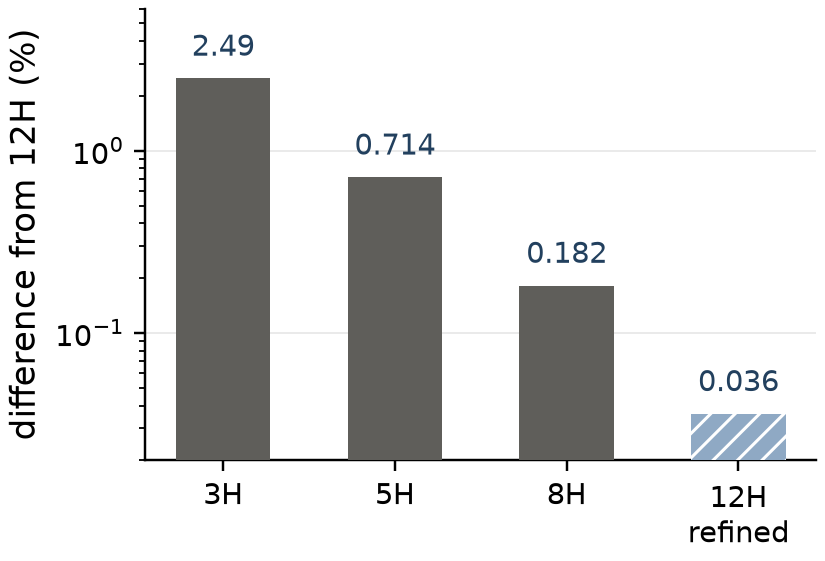
\includegraphics[width=\linewidth]{fig09_truncation.png}
    \end{column}
    \begin{column}{0.46\textwidth}
      \begin{plainsection}{Truncation against the 12H box}
        \begin{tabular}{@{}lrrr@{}}
          \toprule
          & 3H & 5H & 8H\\
          \midrule
          difference & $\TruncThree\%$ & $\TruncFive\%$ & $\TruncEight\%$\\
          \bottomrule
        \end{tabular}
      \end{plainsection}
      \begin{plainsection}{Mesh adequacy, separately}
        Refining the 12H mesh moves it by $\TruncFine\%$ only, so the
        $0.18\%$ is truncation and not mesh noise.
      \end{plainsection}
    \end{column}
  \end{columns}
  \begin{alertblock}{Takeaway}
    Truncation ($\TruncEight\%$) and discretisation ($\ErrSeven\%$) are the same size: quote both.
  \end{alertblock}
\end{frame}

% ---------------------------------------------------------------------
\section{What we submit}
% ---------------------------------------------------------------------

\begin{frame}{The capacitance, with its error bar}
  \begin{columns}[T]
    \begin{column}{0.54\textwidth}
      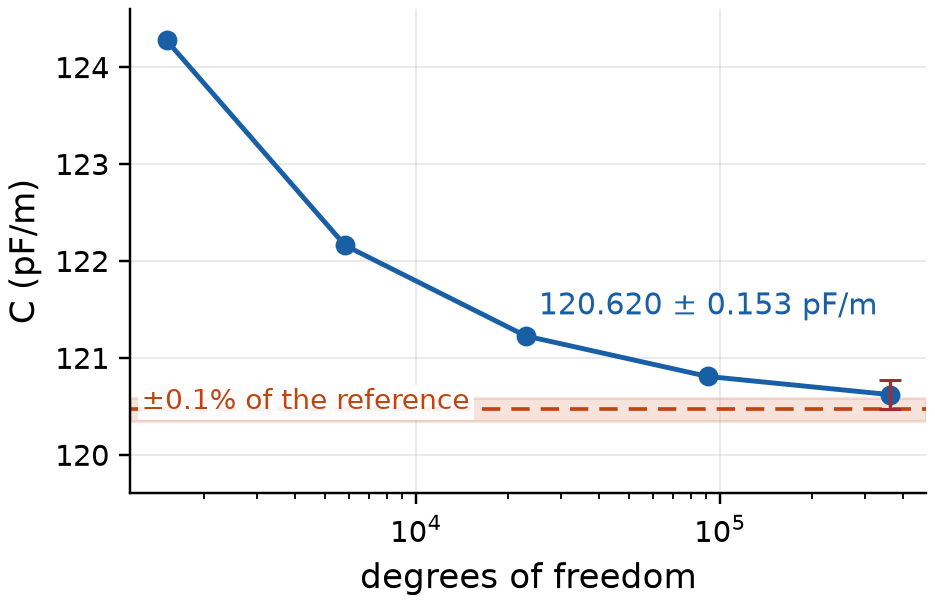
\includegraphics[width=\linewidth]{fig10_final_c.png}
    \end{column}
    \begin{column}{0.42\textwidth}
      \begin{plainsection}{Submitted values}
        \[
          C=\CFinal\pm\CFinalAbs\ \mathrm{pF/m}
        \]
        \[
          \Cair=\CAir\ \mathrm{pF/m}\quad(\text{same M5 $+$ grading mesh})
        \]
        Relative error $\ErrSeven\%$: just outside the $\pm0.1\%$ band.
        M6 was $\ErrSix\%$.
      \end{plainsection}
      \begin{plainsection}{If a cleaner number is wanted}
        The graded mesh gives $\GradedErr\%$ at $\GradedDof$ unknowns; that is
        a different discretisation of the same model, and it is reported as such.
      \end{plainsection}
    \end{column}
  \end{columns}
  \begin{alertblock}{Takeaway}
    This is the number, and this is how far it can be from the truth.
  \end{alertblock}
\end{frame}

\begin{frame}{$\epseff$ and $\Zzero$ are twice as accurate as $C$}
  \centering
  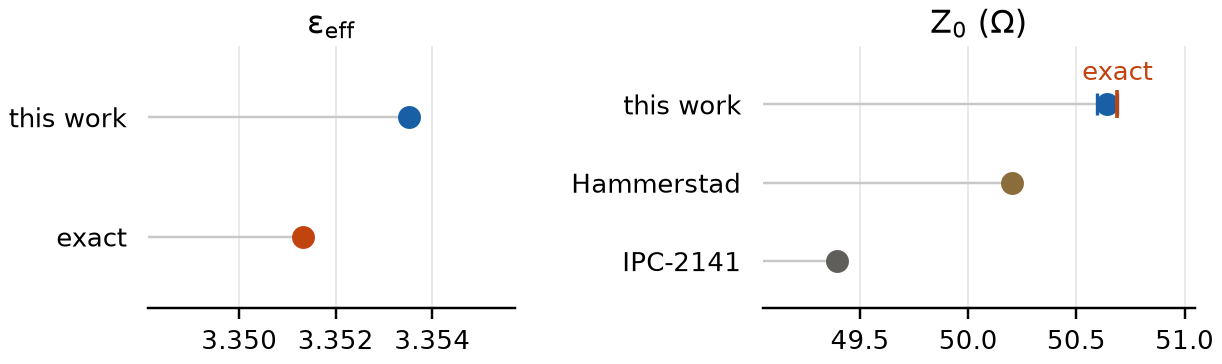
\includegraphics[width=0.84\linewidth]{fig11_engineering.png}
  \vspace{0.25em}
  \begin{columns}[T]
    \begin{column}{0.48\textwidth}
      \begin{plainsection}{The ratio cancels the common bias}
        $\epseff=C/\Cair=\EpsEff$, against an exact $\EpsRef$: an error of
        $\EpsErr\%$, about half the error of $C$ alone.
      \end{plainsection}
    \end{column}
    \begin{column}{0.48\textwidth}
      \begin{plainsection}{Impedance against the benchmarks}
        $\Zzero=1/(c_0\sqrt{C\,\Cair})=\ZFinal\,\Omega$, give or take
        $\ZErrAbs\,\Omega$. Hammerstad gives $\ZHJ\,\Omega$ and IPC-2141
        $\ZIPC\,\Omega$; the two formulas differ by $\ZBenchGap\,\Omega$.
      \end{plainsection}
    \end{column}
  \end{columns}
  \begin{alertblock}{Takeaway}
    Our uncertainty ($\ZErrAbs\,\Omega$) is far smaller than the spread of the formulas we compare with.
  \end{alertblock}
\end{frame}

\begin{frame}{Conclusions}
  \begin{columns}[T]
    \begin{column}{0.48\textwidth}
      \begin{plainsection}{Established}
        \begin{itemize}
          \item The solver is exact to roundoff on $\CheckCount$ analytic cases.
          \item $C_{\rm ref}=\CRef\,\mathrm{pF/m}$, agreed by two elements and
                two codes.
          \item M7 is $\ErrSeven\%$ off, limited by the corner, at order $\OrderPOne$.
          \item Corner grading reaches $\GradedErr\%$ with $\GradedDofFrac\%$ of the unknowns.
        \end{itemize}
      \end{plainsection}
    \end{column}
    \begin{column}{0.48\textwidth}
      \begin{plainsection}{Limits}
        \begin{itemize}
          \item Truncation contributes $\TruncEight\%$, comparable to the
                discretisation error.
          \item \textbf{Quasi-static model}: no losses, no radiation.
          \item The graded mesh is reported as an alternative, not as the
                submitted M7 value.
        \end{itemize}
      \end{plainsection}
    \end{column}
  \end{columns}
  \begin{alertblock}{Takeaway}
    A numerical result is credible when its error, its source and its cure are all visible.
  \end{alertblock}
\end{frame}

\end{document}
